\chapter{Methods and Experiments}%
\label{cha:methods}

\tikzset{zoomnode/.style={rectangle, draw=grey!60, fill=grey!5, very thick, minimum
			width=60mm, minimum height=9mm}}
\tikzset{title/.style={draw=none}}

% TODO: PyTorch, FrEIA
% TODO: Add some intro

\section{Extremal Sampling}%
\label{sec:extremal_sampling}

Since our method relies on sampling outliers in the latent space we will now
examine how this can be accomplished. The latent space is trained to be
approximately gaussian in the case of the normalizing flow, so we can look at
two methods of sampling outliers from a gaussian distribution. Sampling
outliers in the Deep Archetypal Analysis case will be investigated in the next
section.

\subsection{High-Dimensional Gaussian Distributions}%
\label{sub:high_dimensional_gaussian_distributions}
% TODO: Proof?
Since we are working with high-dimensional data, we can investigate the
behavior of random vectors in high dimensions.
Consider the vector $X = (X_1, X_2, \dots, X_d)$ in $\mathbb{R}^d$, where the
coordinates $X_i$ are independently distributed with zero mean and unit
variance. The squared length of vector $X$ is
\begin{equation}%
	\label{eq:square_norm}
	\lVert X \rVert_2^2 = \sum_d X_i^2
\end{equation}
If we assume the coordinates $X_i$ to be standard normally distributed, the
length of the vector is distributed according to a chi distribution with
$d$ degrees of freedom
\begin{equation}%
	\label{eq:sq_norm_chi}
	\lVert X \rVert_2 \sim \chi_d
\end{equation}
If the coordinates are distributed with non-unit variance, $X_i \sim
	\mathcal{N}(0, \sigma^2)$, we similarly get
\begin{equation}%
	\label{eq:sq_norm_chi_sigma}
	\lVert X \rVert_2 \sim \sigma\chi_d
\end{equation}

We can now look at the expected length of the random vector $X$
\begin{equation}
	\begin{aligned}%
		\label{eq:mean_var_sq_dist}
		\mathbb{E} \lVert X \rVert_2   & = \sqrt{2} \frac{\Gamma(\frac{d +
		1}{2})}{\Gamma(\frac{d}{2})}                                            \\
		\mathrm{Var} \lVert X \rVert_2 & = d - (\mathbb{E} \lVert X \rVert_2)^2
	\end{aligned}
\end{equation}
meaning even though the area of highest probability for a high-dimensional
standard normal distribution is close to the origin, most of the mass will be
in a thin, hyperspherical shell with radius $\sim \sqrt{d}$.

If we want to sample from a shell around a high-dimensional standard normal
distribution, we can simply sample coordinates $X_i \sim \mathcal{N}(0,
	\sigma^2)$ and choose $\sigma$ such that a desired radius is reached.

% TODO: Typicality

\subsection{Gumbel Distribution}%
\label{sub:gumbel_distribution}

\begin{figure}[htpb]
	\centering
	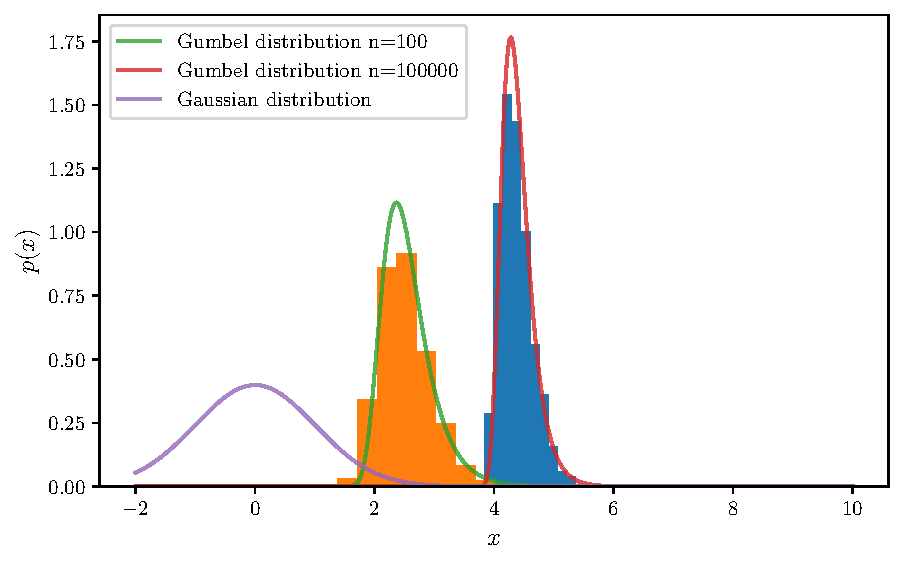
\includegraphics{figures/samples/gumbel_uni.pdf}
	\caption{Gumbel distribution}%
	\label{fig:gumbel_uni}
\end{figure}

Since the latent space is approximately standard normally distributed one way
to approach sampling from outliers is extreme value theory. Extreme value
theory is the theory of the distribution of maxima of sequences of independet,
identically distributed random variables. Let $z_1, \dots, z_n$ be a sequence
of i.i.d. standard normally distributed random variables, then the asymtotic
distribution of the maxima $M_n = \max (z_1, \dots, z_n)$ is
\begin{equation}%
	\label{eq:gumbel_distribution}
	P{a_n ( M_n - b_n ) < x} \rightarrow e^{-e^{-x}}
\end{equation}
where
\begin{equation}
	\begin{aligned}%
		\label{eq:gumbel_params}
		 & a_n = (2 \log n )^{1/2}                                            \\
		 & b_n = (2 \log n )^{1/2} - \frac{1}{2} (2 \log n )^{1/2} (\log \log
		n + \log 4 \pi)
	\end{aligned}
\end{equation}
\citep{leadbetterAsymptoticDistributionsExtremes1983}.

As an example, \autoref{fig:gumbel_uni} shows the distribution of the maxima of
sequences of length $n = 100$ and $n = 100000$ drawn i.i.d. from a standard
normal distribution in comparison.
\begin{figure}[htpb]
	\centering
        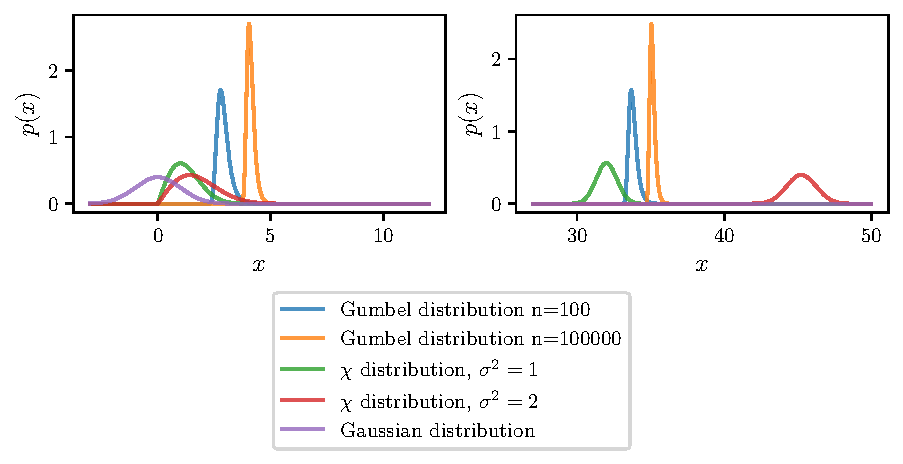
\includegraphics{figures/samples/gumbel_multi.pdf}
	\caption{Comparison of the distribution of the length random vectors
		from a multivariat normal distribution to the Gumbel distribution in
		low and high dimensions.}%
	\label{fig:gumbel_multi}
\end{figure}

This method of sampling outliers is especially useful in lower dimensions, as
we cannot use the methods established in
\autoref{sub:high_dimensional_gaussian_distributions}. We can see in
\autoref{fig:gumbel_multi}, that for $d=2$ the distribution of the lengths of
the random vectors is still rather close to a standard normal distribution, and
indeed doubeling the variance does not lead to a distribution that is noticably
different from the data distribution. For $d=1024$, as is the case for the
image data used for the experiments, we can use the previously introduced
method of sampling from a latent distribution with higher variance, as this
leads to a significantly distinct distribution.

\section{Geometrical Approach}%
\label{sec:geometrical_approach}

In order to make use of the archetype representation of our data we need to
sample archetype coefficients. Sampling from our deep archetypal architecture
can be done as follows. The archetypes, whether they are updated during training
or not, are taken to be fixed and saved. For a fixed configuration of
archetypes the coefficients $a_{ij}$ can be sampled from a Dirichlet distribution,
a generalization of the beta distribution for the multivariate case. For $k$
archetypes and shape parameters $c_i > 0, i = 1, \dots, k$ the probability
density function of the Dirichlet distribution is
\begin{equation}%
	\label{eq:dirichlet_pdf}
	p(a_i) = \frac{ \Gamma ( \sum_j c_j ) }{ \prod_j \Gamma (c_j) } \prod_j
	a_{ij}^{c_j - 1}
\end{equation}
\citep{forbesDirichletDistribution2010}

Since the archetypes are already extreme examples we can control how atypical
the samples should be and furthermore what features we want to be extreme by
controlling the shape parameters.

Once $N$ samples have been drawn we can compute samples from the
$(k-1)$-dimensional latent space.
\begin{equation}%
	\label{eq:aa_k_sample}
	\mathbf{t}_i' = \sum_j a_{ij} \mathbf{z_{j,\mathrm{fixed}}}
\end{equation}

In additon to the layers that map data from the latent space of the invertible
neural network to the archetype space we need to train a layer that
approximates the inverse to this, as a mapping to the $(k-1)$-dimensional
subspace is in general not invertible. The layer is chosen to be a linear layer
with no activation function, details on how this layer is trained can
be found in \autoref{sec:network_architecture}
\begin{equation}%
	\label{eq:aa_upsample}
	\mathbf{t}_i = f_C (\mathbf{t}_i')
\end{equation}
Finally we can use the neural network to get samples in data space
\begin{equation}%
	\label{eq:aa_to_data}
	\mathbf{x}_i = \mathrm{INN}^{-1} (\mathbf{t}_i)
\end{equation}

Additional modifications can be applied: We can add gaussian noise to the
samples in any of the latent spaces to get more variation or more extreme
samples. Another idea is to change the constraint on the coefficients to be
quadratic, but initial tests have proven unsuccessful so this approch was not
investigated further.

Another modification is to add a random sample to $\mathbf{t}_i$ from the
nullspace of the mapping to the archetype space to mitigate the loss of
information that occures. Ignoring the additional softmax activation the
mapping of the data onto archetype coefficients is linear. If $M_A$ is the
matrix of the weights of this linear network layer, the mapping can be
described as
\begin{equation}%
	\label{eq:aa_mapping}
	\mathbf{a}_i = M_A \mathbf{t}_i
\end{equation}
where $\mathbf{a}_i$ are the resulting archetype coefficients for data vector
$\mathbf{t}_i$. Mapping archetype coefficients back into the latent space of
the network can then be thought of as solving this linear equation for
$\mathbf{t}_i$. However, in general a solution $\mathbf{t}'_i$ to this linear
equation is not unique and
\begin{equation}
	\mathbf{t}''_i = \mathbf{t}'_i + \mathbf{k}
\end{equation}
is another solution to the equation. Here, $\mathbf{k}$ is a vector from the
kernel or nullspace of $M_A$, the space of all vectors that are solutions to
$M_A \mathbf{x} = \mathbf{0}$. All solutions to \autoref{eq:aa_mapping} are
given by
\begin{equation}%
	\label{eq:linear_all_solutions}
	\mathbf{t}_i = M_A^+ \mathbf{a}_i + [I - M_A^+ M_A] \mathbf{w}
\end{equation}
where $\mathbf{w}$ is an arbitrary $d$-dimensional vector and $M_A^+ =
	(M_A^\top M_A)^{-1} M_A^\top$ is the Moore-Penrose inverse of
$M_A$~\citep{jamesGeneralisedInverse1978}. As in our case the mapping is not
linear but has an additional softmax activation we cannot use this result as
is. However, since we train this whole setup to be invertible via the linear
mapping $f_C$ the approximation is close enough to still improve the results of
the sampling, as shown in \autoref{sub:nullspace_sampling}. We simply augment
the result of $f_C$ similarly to \autoref{eq:linear_all_solutions} using $M_A$
as if no softmax was applied
\begin{equation}%
	\label{eq:augmented_t}
	\mathbf{t}'_i = f_C(\mathbf{a}_i) + [I - M_A^+ M_A] \mathbf{w}
\end{equation}
where $\mathbf{w}$ is sampled from the latent space distribution of the
normalizing flow.

\section{Discriminator Training}%
\label{sec:discriminator_training}

To investigate if our methods of generating outliers can be used in practice we
train a discriminator to distinguish inlier samples from outliers and test it
on other outlier data. The availability of other outlier data that resembles
the inlier data is one of the reasons we chose EMNIST as one of our datasets,
as discussed in \autoref{sec:datasets}.

The architecture of the discriminator neural network modeled after the
DCGAN architecture~\citep{radfordUnsupervisedRepresentationLearning2016} with
additional inputs to make the discriminator class
conditional~\citep{mirzaConditionalGenerativeAdversarial2014}. In detail, the
discriminator consists of two small networks of one strided convolution each
with leaky rectified linear unit activations that process the image input and
the condition respectively. The outputs of these two networks are concatenated
and fed into two convolutional layers with leaky rectified linear unit
activations and batch
normalization~\citep{ioffeBatchNormalizationAccelerating2015}. Finally a last
convolutional layer with the sigmoid function as activation is applied.
For samples from the data distribution $x \sim p_{\mathrm{in}}$ with class
labels $y$ and some outlier outlier distribution (e.g. from using the change of variables formula
for an outlier distribution of a normalizing flow) $z \sim p_{\mathrm{out}}$
the discriminator $D$ is trained to maximize
\begin{equation}
	\mathbb{E}_{\hat{x}, \hat{y} \sim p_{\mathrm{in}}} \log D(x, y) +
	\mathbb{E}_{z \sim p_{\mathrm{out}}} \log ( 1 - D(z, y) )
\end{equation}
where the class labels for the outliers are sampled from a uniform distribution
over all class labels.

\begin{figure}[htpb]
	\begin{center}
		\begin{tikzpicture}[scale=1, transform shape]
			\node (in) [] {Image $(n_{\mathrm{Batch}} \times n_{\mathrm{Channels}} \times 32 \times 32)$};

			\node (il1) [zoomnode, below=0.4cm of in]  {Conv $4 \times 4$, 64, /2};
			\node (il2) [zoomnode, below=0.4cm of il1] {LeakyReLU};
			\node (il3) [zoomnode, below=0.4cm of il2]  {Dropout $0.2$};

			\node (cin) [right=of in] {Condition $(n_{\mathrm{Batch}} \times n_{\mathrm{Classes}} \times 32 \times 32)$};

			\node (cl1) [zoomnode, below=0.4cm of cin]  {Conv $4 \times 4$, 64, /2};
			\node (cl2) [zoomnode, below=0.4cm of cl1] {LeakyReLU};

			\node (l1) [zoomnode]
                            at ($ (0,0)!(il3.south)!(0,1) + (0,-1.2cm) + ($(0,0)!(il3)!(1,0)$)!0.5!($(0,0)!(cl2)!(1,0)$)$)
                            {Conv $4 \times 4$, 256, /2};
			\node (l2) [zoomnode, below=0.4cm of l1] {BatchNorm};
			\node (l3) [zoomnode, below=0.4cm of l2] {LeakyReLU};
			\node (l4) [zoomnode, below=0.4cm of l3]  {Dropout $0.2$};
                        \node (l5) [zoomnode, below=0.4cm of l4]  {Conv $4
                            \times 4$, 128, /2};
			\node (l6) [zoomnode, below=0.4cm of l5] {BatchNorm};
			\node (l7) [zoomnode, below=0.4cm of l6] {LeakyReLU};
			\node (l8) [zoomnode, below=0.4cm of l7]  {Dropout $0.2$};
			\node (l9) [zoomnode, below=0.4cm of l8]  {Conv $4
                            \times 4$, 1, /2};

			\node (out) [below=0.4cm of l9] {Output
                            $(n_{\mathrm{Batch}} \times 1)$};

			\draw[grapharrow] (in)   -- (il1);
			\draw[grapharrow] (il1)   -- (il2);
			\draw[grapharrow] (il2)   -- (il3);
			\draw[grapharrow] (cin)   -- (cl1);
			\draw[grapharrow] (cl1)   -- (cl2);

                        \draw[grapharrow] (il3.south) |- ($ (l1.north) + (0,0.4cm) $) -| (l1);
                        \draw[grapharrow] (cl2.south) |- ($ (l1.north) + (0,0.4cm) $) -| (l1);

			\draw[grapharrow] (l1)   -- (l2);
			\draw[grapharrow] (l2)   -- (l3);
			\draw[grapharrow] (l3)   -- (l4);
			\draw[grapharrow] (l4)   -- (l5);
			\draw[grapharrow] (l5)   -- (l6);
			\draw[grapharrow] (l6)   -- (l7);
			\draw[grapharrow] (l7)   -- (l8);
			\draw[grapharrow] (l8)   -- (l9);
			\draw[grapharrow] (l9)   -- (out);
		\end{tikzpicture}
	\end{center}
	\caption{Architecture of the invertible neural network. The number of
		coupling blocks in each section is specific to the experiments and
		mentioned there.}%
	\label{fig:disc_architecture}
\end{figure}

% Classifier
Another application is to use the generated outliers to train a classifier to
have high confidence on inliers and show low confidence otherwise. Lee et al.
propose training a generative adversarial network jointly with such a
classifier and use the generator network to create outlier
samples~\citep{leeTrainingConfidencecalibratedClassifiers2018}. Since we do not
need to train a generator jointly with the classifier we simply use our methods
of outlier generation and train the classifier similarly to the classifier
update step of Lee et al. The classifier shows low confidence when the
distribution over class labels is close to a uniform distribution. We can
compute the Kullback-Leibler divergence to get a measure for how close these
two distributions are.  For samples from the data distribution $x \sim
	p_{\mathrm{in}}$ with class labels $y$ and some outlier outlier distribution $z
	\sim p_{\mathrm{out}}$ the classifier is trained to maximize
\begin{equation}
	\mathbb{E}_{\hat{x}, \hat{y} \sim p_{\mathrm{in}}} \log p(y=\hat{y} | \hat{x}) -
	\beta \mathbb{E}_{z \sim p_{\mathrm{out}}} \mathrm{KL}(\mathcal{U}(y) | p(y | z))
\end{equation}
where $\beta$ is a hyperparameter that weights the two loss terms. Except for
the toy example we use a VGG11 model as the classification
network~\citep{simonyanVeryDeepConvolutional2015}.

\section{Network Architecture}%
\label{sec:network_architecture}

\begin{figure}[htpb]
	\begin{center}
		\begin{tikzpicture}[scale=1, transform shape]
			\node[varnode] (x) {$x$};
			\node[opnode] (inn) [right=of x] {INN};
			\node[varnode] (t) [right=of inn] {$t$};

			\node[opnode] (fa) at ($ (t) + (2cm,1cm) $) {$f_A$};
			\node[opnode] (fb) at ($ (t) + (2cm,-1cm) $) {$f_B$};

			\node[varnode] (A) [right=of fa] {$A$};
			\node[varnode] (B) [right=of fb] {$B$};

			\draw[grapharrow] (x)   -- (inn);
			\draw[grapharrow] (inn)   -- (t);
			\draw[grapharrow] (t)   -- (fa);
			\draw[grapharrow] (t)   -- (fb);
			\draw[grapharrow] (fa)   -- (A);
			\draw[grapharrow] (fb)   -- (B);
		\end{tikzpicture}
	\end{center}
	\caption{Forward pass of the normalizing flow with additional layers
		for the mapping to archetype coefficients.}%
	\label{fig:inn_aa_forward}
\end{figure}

\begin{figure}[htpb]
	\begin{center}
		\begin{tikzpicture}[scale=1, transform shape]
			\node[varnode] (x) {$x$};
			\node[opnode] (inn) [right=of x] {INN};
			\node[varnode] (t) [right=of inn] {$t$};

			\node[opnode] (fc) [right=of t] {$f_C$};

			\node[varnode] (ta) [right=of fc] {$t'$};

			\draw[grapharrow] (ta)   -- (fc);
			\draw[grapharrow] (fc)   -- (t);
			\draw[grapharrow] (t)   -- (inn);
			\draw[grapharrow] (inn)   -- (x);
		\end{tikzpicture}
	\end{center}
	\caption{Inverse computation from lower dimensional sample created from
		archetype coefficients to data space.}%
	\label{fig:inn_aa_backward}
\end{figure}


\begin{figure}[htpb]
	\begin{center}
		\begin{subfigure}[]{0.45\textwidth}
			\begin{center}
				\begin{tikzpicture}[scale=1, transform shape]
					\node (in) [] {Image $(n_{\mathrm{Channels}} \times 32 \times 32)$};

					\node (inn) [title, below=0.4cm of in, text width=60mm, align=left] {INN};

					\node (d1) [zoomnode, below=0.4cm of inn]  {Downsampling Layer};
					\node (c1) [zoomnode, below=0.4cm of d1] {High-Res Conv Coupling Blocks};
					\node (d2) [zoomnode, below=0.4cm of c1]  {Downsampling Layer};

					\node (c2) [zoomnode, below=0.4cm of d2] {Low-Res Conv Coupling Blocks};
					\node (d3) [zoomnode, below=0.4cm of c2]  {Flattening Layer};

					\node (c3) [zoomnode, below=0.4cm of d3] {Linear Coupling Blocks};
					\node (out) [below=0.4cm of c3] {Latent Vector $(n_{\mathrm{Channels}} \cdot 1024)$};

					\node [draw=red!60, inner sep=0.1cm, fit={(inn) (d1) (c1) (d2) (c2) (d3) (c3)}] {};

					\draw[grapharrow] (in)   -- (d1);
					\draw[grapharrow] (d1)   -- (c1);
					\draw[grapharrow] (c1)   -- (d2);
					\draw[grapharrow] (d2)   -- (c2);
					\draw[grapharrow] (c2)   -- (d3);
					\draw[grapharrow] (d3)   -- (c3);
					\draw[grapharrow] (c3)   -- (out);
				\end{tikzpicture}
			\end{center}
		\end{subfigure}
		\begin{subfigure}[]{0.45\textwidth}
			\begin{center}
				\begin{tikzpicture}[scale=1, transform shape]
					\node (in) [] {Input $(2 \cdot n_{\mathrm{Channels}} \times 16 \times 16)$};

					\node (inn) [title, below=0.4cm of in, text width=60mm,
						align=left] {Conv Coupling \\ Function};

					\node (d1) [zoomnode, below=0.4cm of inn]  {Conv $3 \times 3$, 16};
					\node (c1) [zoomnode, below=0.4cm of d1] {ReLU};
					\node (d2) [zoomnode, below=0.4cm of c1]  {Conv $3 \times 3$, 16};

					\node (c2) [zoomnode, below=0.4cm of d2] {ReLU};
					\node (d3) [zoomnode, below=0.4cm of c2]  {Conv $3 \times 3$, $4 \cdot n_{\mathrm{Channels}}$};

					\node (out) [below=0.4cm of d3] {Output $(4 \cdot n_{\mathrm{Channels}} \times 16 \times 16)$};

					\node [draw=red!60, inner sep=0.1cm, fit={(inn) (d1) (c1) (d2) (c2) (d3)}] {};

					\draw[grapharrow] (in)   -- (d1);
					\draw[grapharrow] (d1)   -- (c1);
					\draw[grapharrow] (c1)   -- (d2);
					\draw[grapharrow] (d2)   -- (c2);
					\draw[grapharrow] (c2)   -- (d3);
					\draw[grapharrow] (d3)   -- (out);
				\end{tikzpicture}
			\end{center}
		\end{subfigure}
	\end{center}
	\caption{Architecture of the invertible neural network. The number of
		coupling blocks in each section is specific to the experiments and
		mentioned there.}%
	\label{fig:inn_contents}
\end{figure}

% Architecture of the INN
The architecture of the invertible neural network consists of a series of
affine coupling blocks as discussed in \autoref{sub:coupling_layers}. The
coupling functions are a series of three layers of either convolutions or
linear mappings with rectified linear activation functions. Between sets of
coupling layers downsampling is applied. The actual configuration of these
components is specific to the experiments and mentioned in the respective
subsections.

As described in \autoref{sub:normalizing_flows} the network is train to
minimize the negative log-likelihood of the training data.

To map from the latent space to the archetype coefficient $a_{ij}$ and $b_{ji}$
one linear layer with softmax activation each is used, denoted as $f_A$ and
$f_B$ respectively. Since this is in general not invertible, we additionally
train a linear layer without activation function $f_C$ to map back from this
low dimensional space to the latent space of the normalizing flow. For this,
the whole setup is trained to minimize the mean squared reconstruction error in
addition to the optimization problem shown in \autoref{eq:archetype_rss}.

% TODO: ADAM
% TODO: GLOW design
% TODO: every other low-res conv is 1x1

\section{Datasets}%
\label{sec:datasets}

In the our experiments we use multiple different datasets. The first dataset is the
EMNIST dataset~\citep{cohenEMNISTExtensionMNIST2017}, an extension to the MNIST
dataset of handwritten digits~\citep{lecunGradientbasedLearningApplied1998}. It
consists of greyscale images of handwritten digits and letters that are $28
	\times 28$ pixels in size. For easier use in the experiments and consistency
across all datasets the images are zero-padded to a size of $32 \times 32$
pixels. In the rest of the work, we will refer to the set of images of digits
as the digits dataset and to the set of letters as the letters dataset.
As an additonal source of outliers, we use the
Fashion-MNIST~\citep{xiaoFashionmnistNovelImage2017} and
Kuzushiji-MNIST~\citep{clanuwatDeepLearningClassical2018} datasets, referred to
as the fashion dataset and the KMNIST dataset in the rest of this work. The
fashion dataset consists of greyscale images of clothing that are $28 \times
	28$ pixels in size and again zero-padded to $32 \times 32$ pixels. The KMNIST
dataset contains greyscale images of cursive Japanese characters, again they
are $28 \times 28$ pixels in size and zero-padded.
To investigate our methods on slightly more complex images, we use the Facial
Expression Research Group-Database~\citep{anejaModelingStylizedCharacter2017a},
a set of images of six animated, stylized characters with seven different
facial expressions. The $256 \times 256$ pixel images are resized to $32 \times
	32$ pixels. In the rest of the work, we refer to this dataset, using the
characters as classes, as the people dataset. Since there is no dataset that
provides equally closely related outliers for the people dataset as for the
digits dataset, we use the CIFAR10
dataset~\citep{krizhevskyLearningMultipleLayers2009} of color images as a
substitute. For all datasets, the number of samples in the training and test
split as well as the number of classes is listed in \autoref{tab:datasets}.

\begin{table}[htpb]
	\centering
	\caption{caption}
	\label{tab:datasets}
	\begin{tabular}{lrrr}
\toprule
{} & {# Classes} & {Training} & {Test} \\
{Dataset} & {} & {} & {} \\
\midrule
digits & 10 & 240000 & 40000 \\
letters & 26 & 124800 & 20800 \\
fashion & 10 & 60000 & 10000 \\
KMNIST & 10 & 60000 & 10000 \\
people & 6 & 55766 & \\
CIFAR10 & 10 & 50000 & 10000 \\
\bottomrule
\end{tabular}

\end{table}
% TODO: replace dataset names
